\clearpage
\newpage
\chapter{Background Estimation}
\label{sec:bsbackgroundEstimation}
The primary sources of Standard Model background for this analysis are QCD multijet and $\ttbar$ production. 
The shape of the $\ttbar$ contribution to the background is taken from Monte Carlo, and the normalization is derived from data by using a $\ttbar$ rich control region.  The QCD multijet 
background contribution is derived from data by inverting the W candidate mass requirement for W-tagging.

\section{QCD Background Estimation}
\label{sec:bssideband}
\label{sec:bsqcdBackgroundEstimationProcedure}
In order to extract the QCD multijet background contribution, we determine the mistagging rate for the CMS top tagging algorithm (see Section \ref{sec:toptagging}).  
To measure this top mis-tagging rate, we turn to a control region based on inverting the W-tagging mass requirement.  We look in a W candidate mass window around of the signal region 
requirement ($30~\GeV < M_{jet} < 70~\GeV$ or $100~\GeV < M_{jet}$). 

After applying this selection, we take the inverse ratio of top candidate jets to top candidate jets that are top-tagged to define the top-mistagging rate.  
To keep the kinematics similar in the sideband and similar region when reconstructing $\mathrm{M_{tW}}$, the top candidate mass requirement is kept on the jets in both regions.  
To extract a QCD background estimate, we weight the events that pass the W-tagging requirements in the full selection by the top-mistagging rate.

The parameterization of the top-mistagging rate is two dimensional and considers both the $|\eta|$ and $\pt$ of the top candidate jets.  
We break down data into two distinct regions in $|\eta|$. 


\begin{itemize}
	\item \text{Low} $(0.0 < |\eta| \leq 1.0)$
	\item \text{High} $(1.0 < |\eta| \leq 2.4)$ 
\end{itemize}

The regions in $|\eta|$ are then individually parameterized in $\pt$ to produce the average top-mistagging rate.  We perform this parameterization 
of the top-mistagging rate in an attempt to constrain the kinematic correlations inherent in top-tagging.

To smooth out the binning of the average top-mistagging rate, a study of functional fits was conducted for the top-mistagging rate (see Figure \ref{figs:bsBKGFITCOMP}).
We use the same functional form for the top-mistagging rate fit as the average b-tagging rate in the $\wpr$ search (see Section~\ref{sec:qcdBackgroundEstimationProcedure})
with the bifurcation points set to be 640$~\GeV$ and 590$~\GeV$ for the low and high $\eta$ regions respectively.

The errors on the top-mistagging rate are then extracted using the full covariance matrix as obtained from output of the fitting 
algorithm.   
Additionally, we assign a systematic uncertainty to cover the choice of the fit function (see Section \ref{sec:bssystematics}) 
based on several alternative functional forms.
Figure \ref{figs:bstagsandprobes8TeV} shows the tags (numerator) and probes (denominator) of the top-mistagging rate.
Figure \ref{figs:bstagrateetafit} shows the two fitted top-mistagging rates parameterized in $\pt$.  

In the creation of the top-mistagging rate, $\ttbar$ is subtracted using the prescription outlined in Section~\ref{sec:ttSubtraction}
\begin{figure}[htcb]
\centering
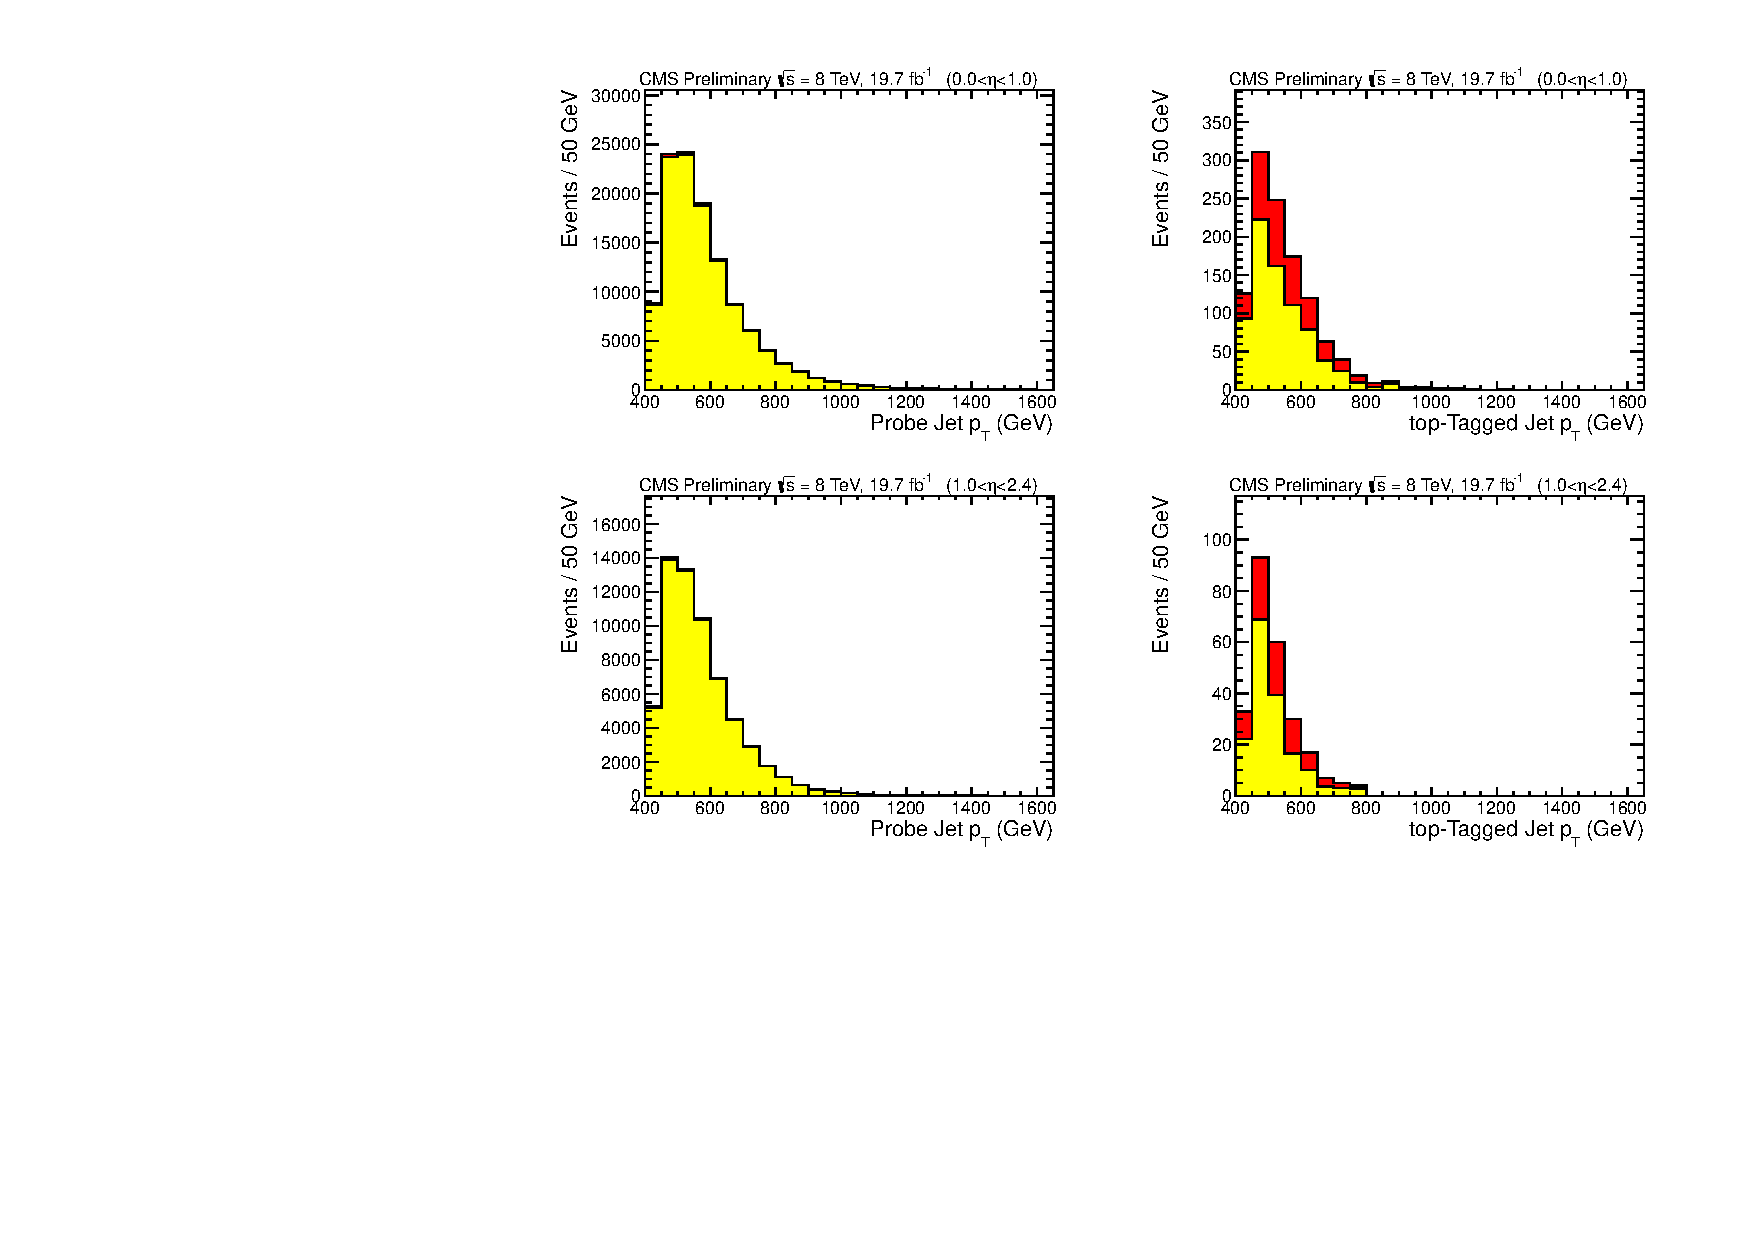
\includegraphics[width=1.0\textwidth]{AN-14-049/figs/tagsandprobes}
\caption{The tags and probes used for the average top-mistagging rate for the two regions in $|\eta|$.  
Here, tags are the numerator and probes are the denominator of the average top-mistagging rate}
\label{figs:bstagsandprobes8TeV}
\end{figure}

\begin{figure}[htcb]
\begin{center}
\subfigure{\label{figs:bstagrateeta1fit}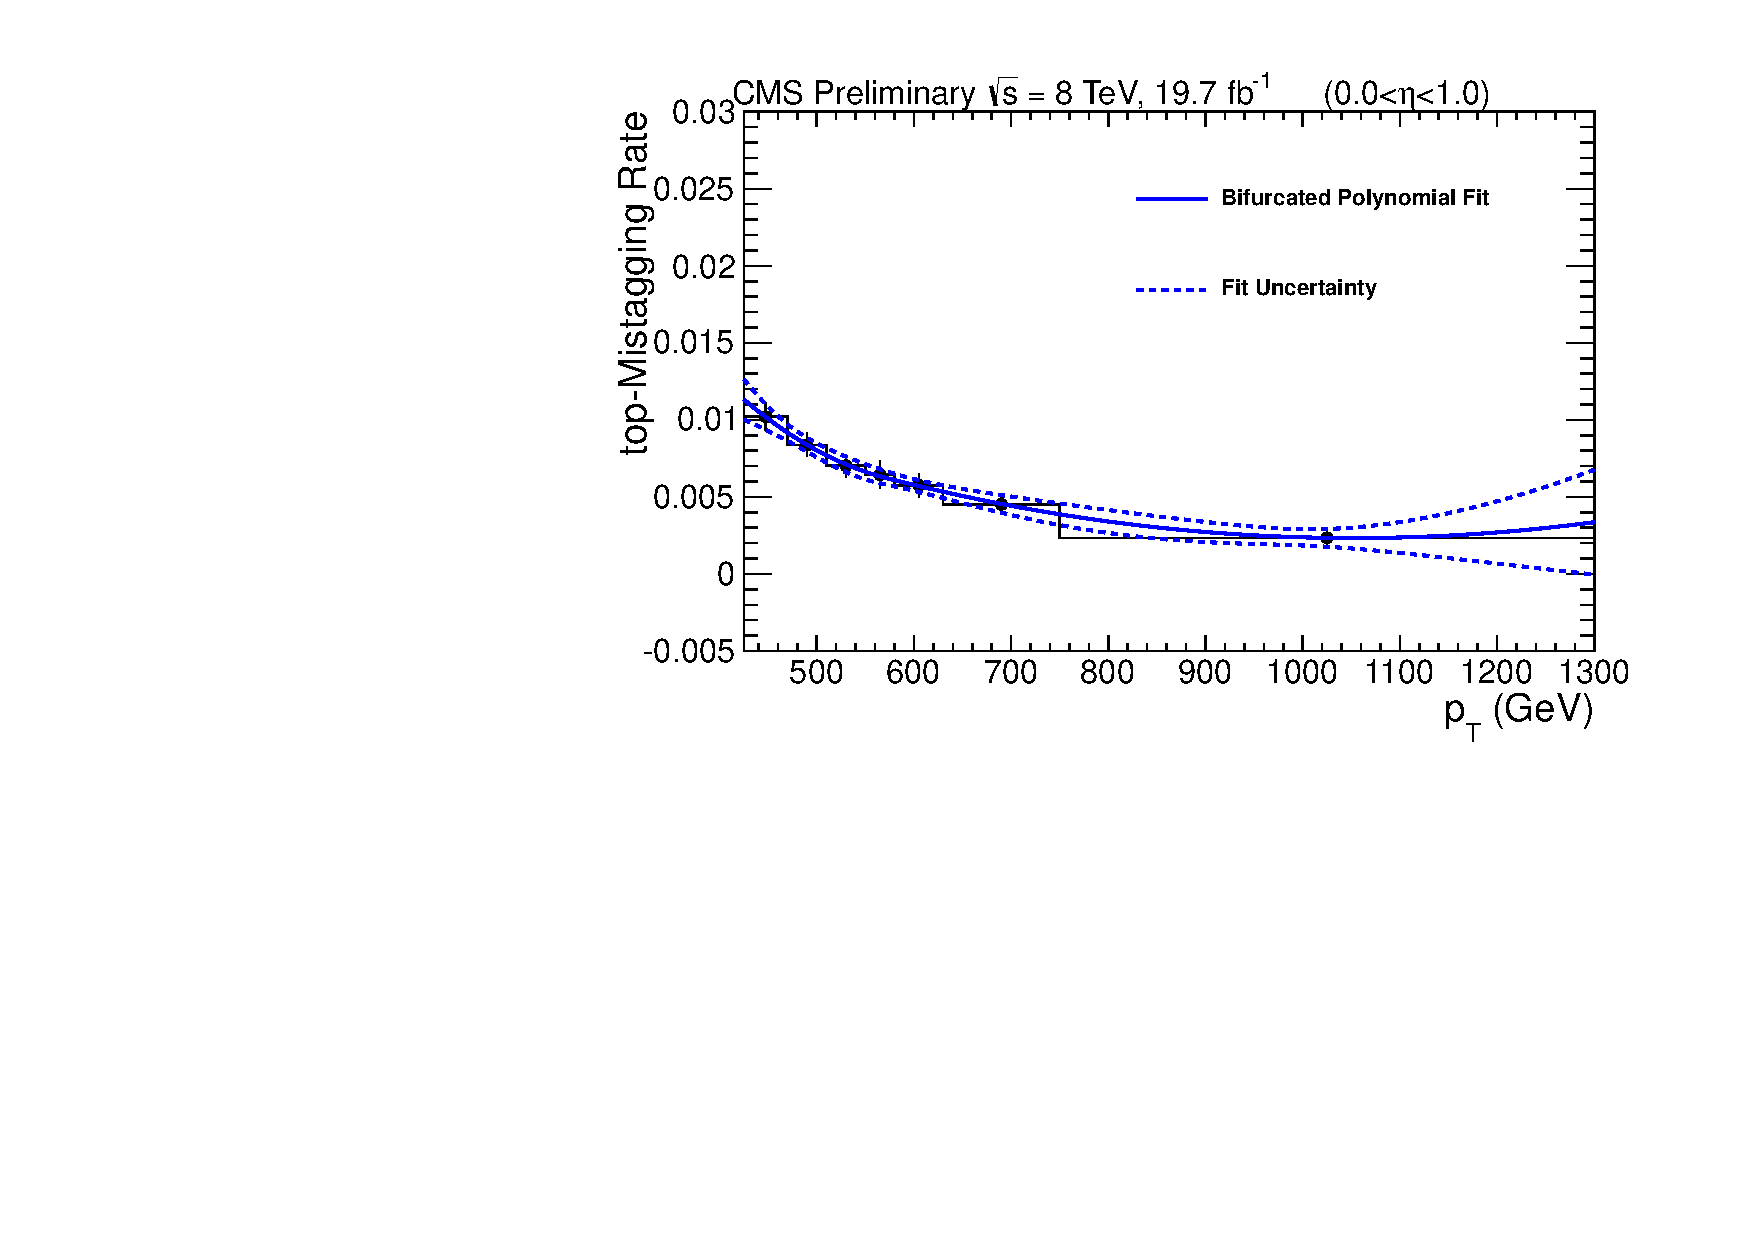
\includegraphics[width=0.75\textwidth]{AN-14-049/figs/tagrateeta1fitBP.pdf}}\\
\subfigure{\label{figs:bstagrateeta2fit}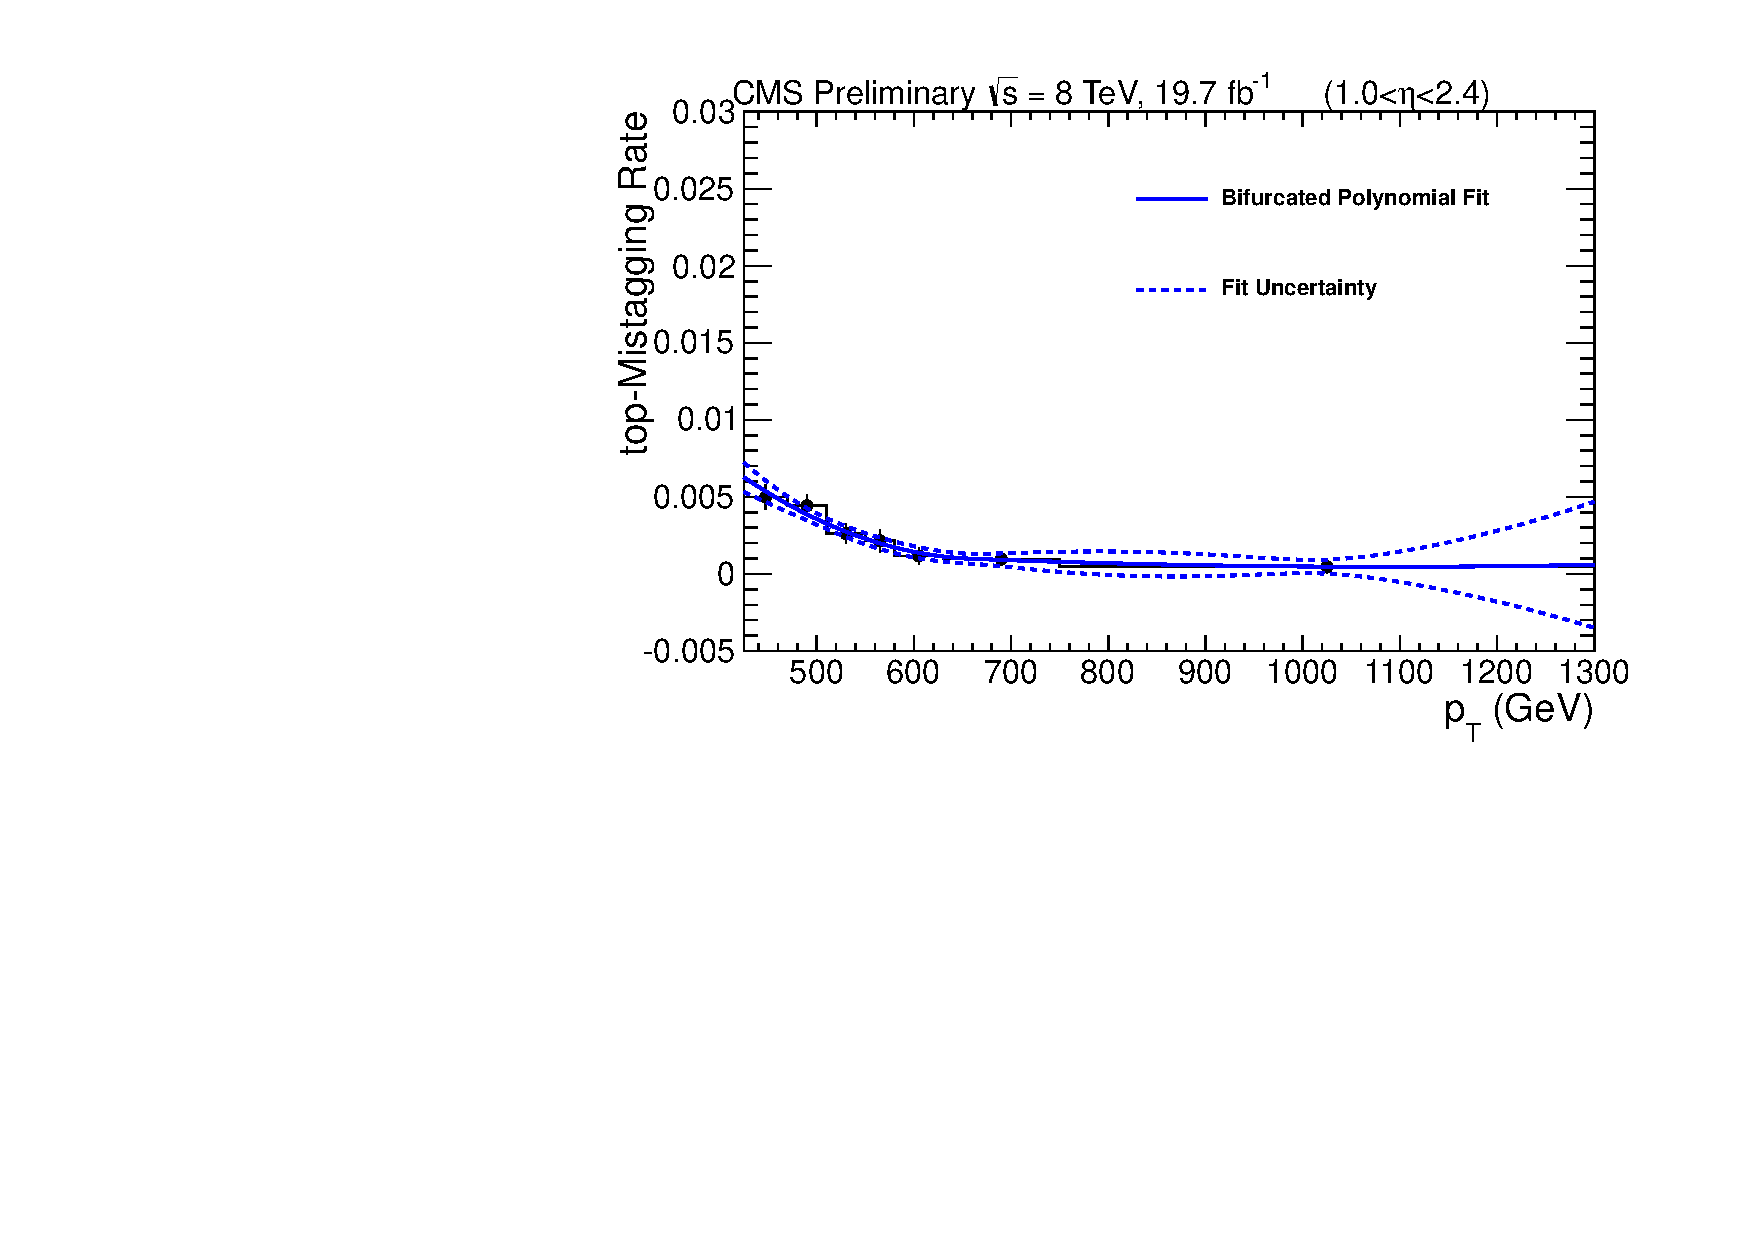
\includegraphics[width=0.75\textwidth]{AN-14-049/figs/tagrateeta2fitBP.pdf}}\\
\caption{
$\pt$ parameterized average top-mistagging rate from the low (top) and high (bottom) $\eta$ regions. 
the top-mistagging rate is shown in black, the polynomial fit is shown in blue, and the propagated errors from the fit are shown as a blue dashed line.}
\label{figs:bstagrateetafit}
\end{center}
\end{figure}



\begin{table}
\begin{center}
\bf{Background Composition}\\
\begin{tabular}{|c||c|c|}
\hline
\bf{region} & \bf{pre top-tag}  & \bf{post top-tag} \\
\hline
signal region QCD & 37801  & 211 \\
\hline
signal region $\ttbar$ & 457 & 129 \\
\hline
sideband region QCD & 176741 & 926 \\
\hline
sideband region $\ttbar$ & 1758 & 456 \\
\hline
\end{tabular}
\end{center}
\caption{expected QCD and $\ttbar$ yields in the signal region and sideband used for extracting the top-mistagging rate.  The QCD expected events are measured after $\ttbar$ subtraction.}
\label{table:bsbkgcomp}
\end{table}


\section{Top Candidate Mass Correction}
\label{sec:bsmodmass}
The application of the top-mistagging rate on the pre top-tagged sample provides a close approximation of the shape and normalization of the signal region.  
However, there is a known shape based discrepancy in the modeling of the top-candidate jet mass (see \cite{7tevZprime}). 
Before the number of subjets and minimum pairwise mass requirements, the QCD top candidate mass spectrum is a rapidly falling function, whereas after 
this selection the QCD top candidate mass spectrum is nearly flat.  To investigate this discrepancy, we take the top candidate mass 
spectrum from QCD Monte Carlo before and after the number of subjets, minimum pairwise mass, and N-subjettiness requirements.  
The ratio of these normalized templates gives an approximate correction for this effect (see Figure \ref{figs:bsmodmass}).  The uncertainty for this procedure is taken as half the correction.  
The correction and uncertainty are both interpolated to roughly correct for binning.  This correction can be seen for data in Figure \ref{figs:bsdatatmass}

The effect of this correction on the $M_{tW}$ and top candidate $\pt$ templates can be seen in figure \ref{figs:bsmodmasseffect}.

\begin{figure}[Htcb]
\centering
\subfigure{\label{figs:bsqcdtmass}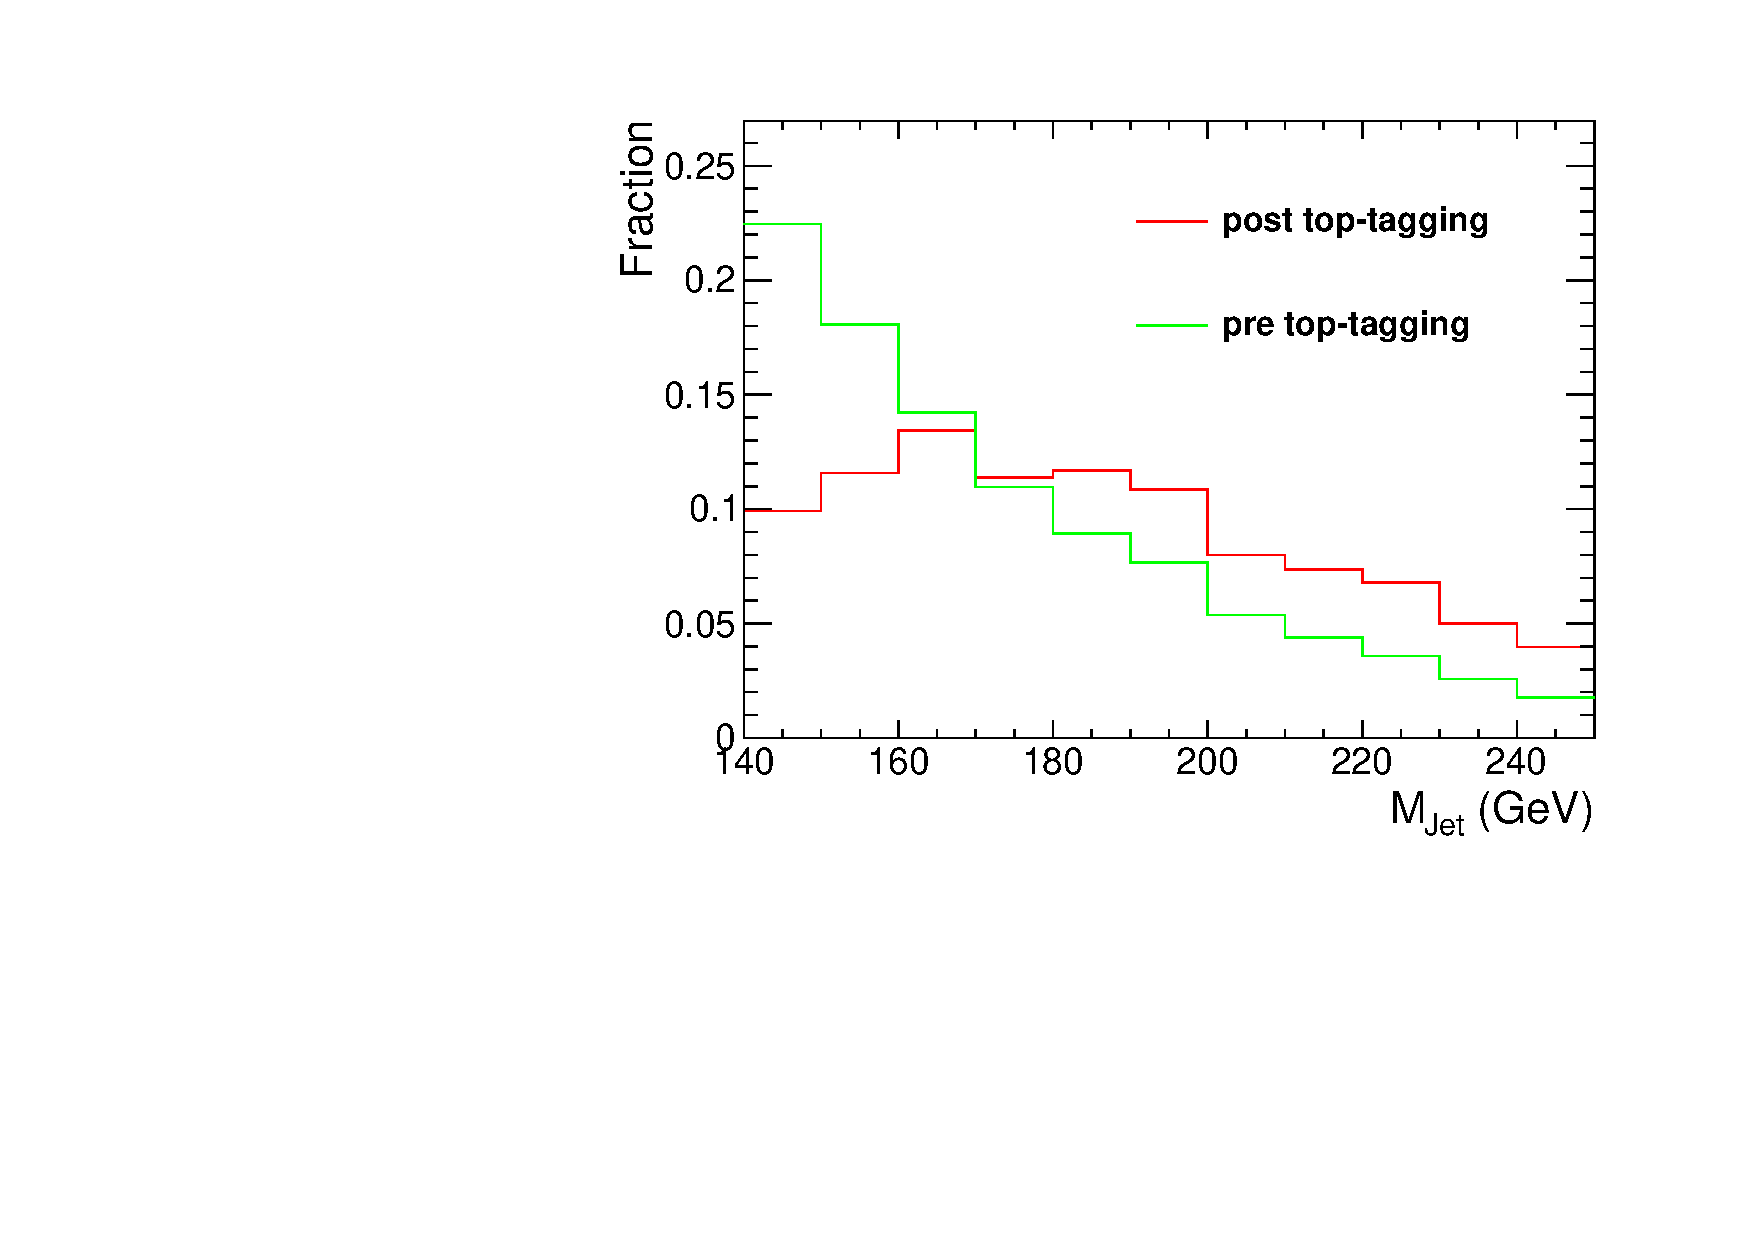
\includegraphics[width=.7\textwidth]{AN-14-049/figs/QCDtmasscomp.pdf}}\\
\subfigure{\label{figs:bsmodmassplot}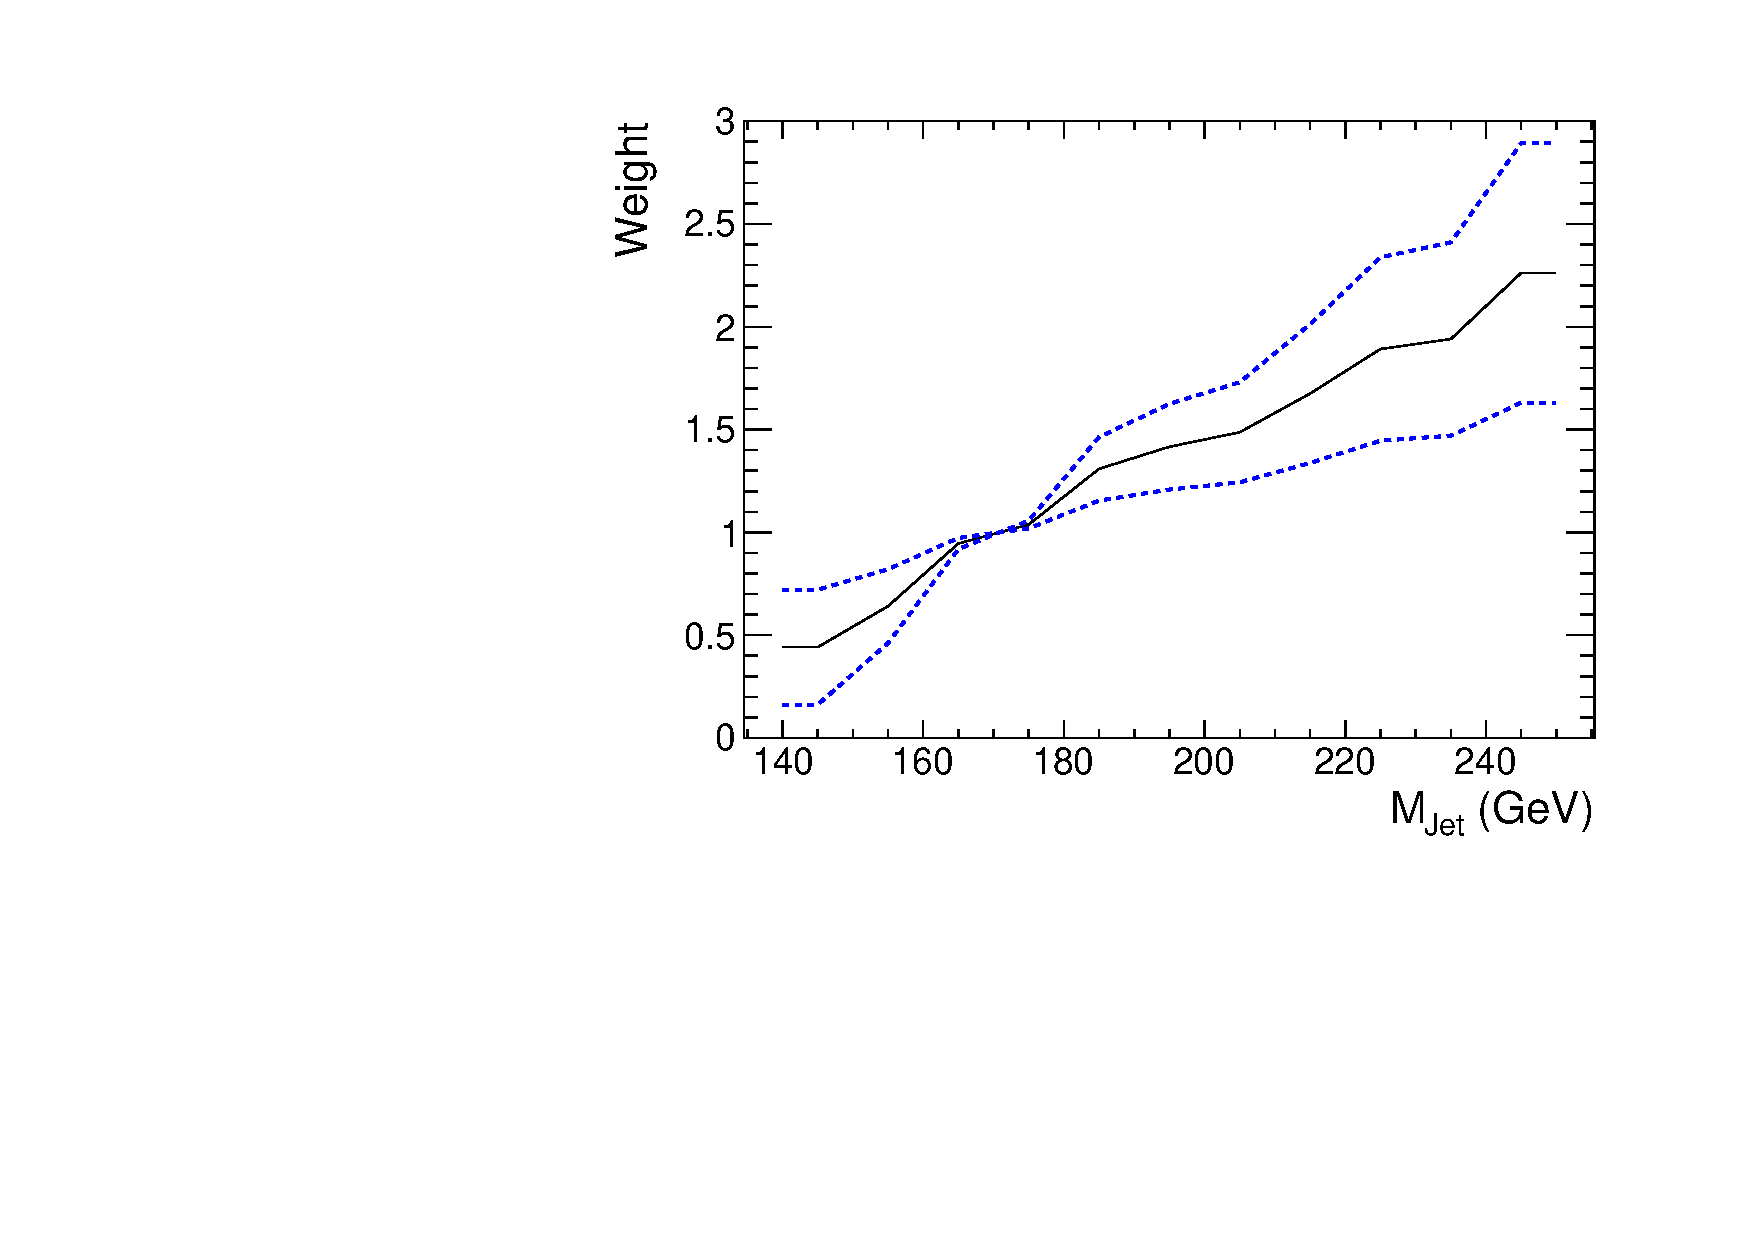
\includegraphics[width=.7\textwidth]{AN-14-049/figs/ModmassPlot.pdf}}
\caption{A plot of the top candidate mass spectrum in QCD Monte Carlo before and after top-tagging (top).  The correction used for this 
discrepancy (bottom) created by dividing the templates in the top plot.  The uncertainty used for this correction is shown as the blue dashed line.}
\label{figs:bsmodmass}
\end{figure}

\begin{figure}[Htcb]
\centering
\subfigure{\label{figs:bsdatatmassplot}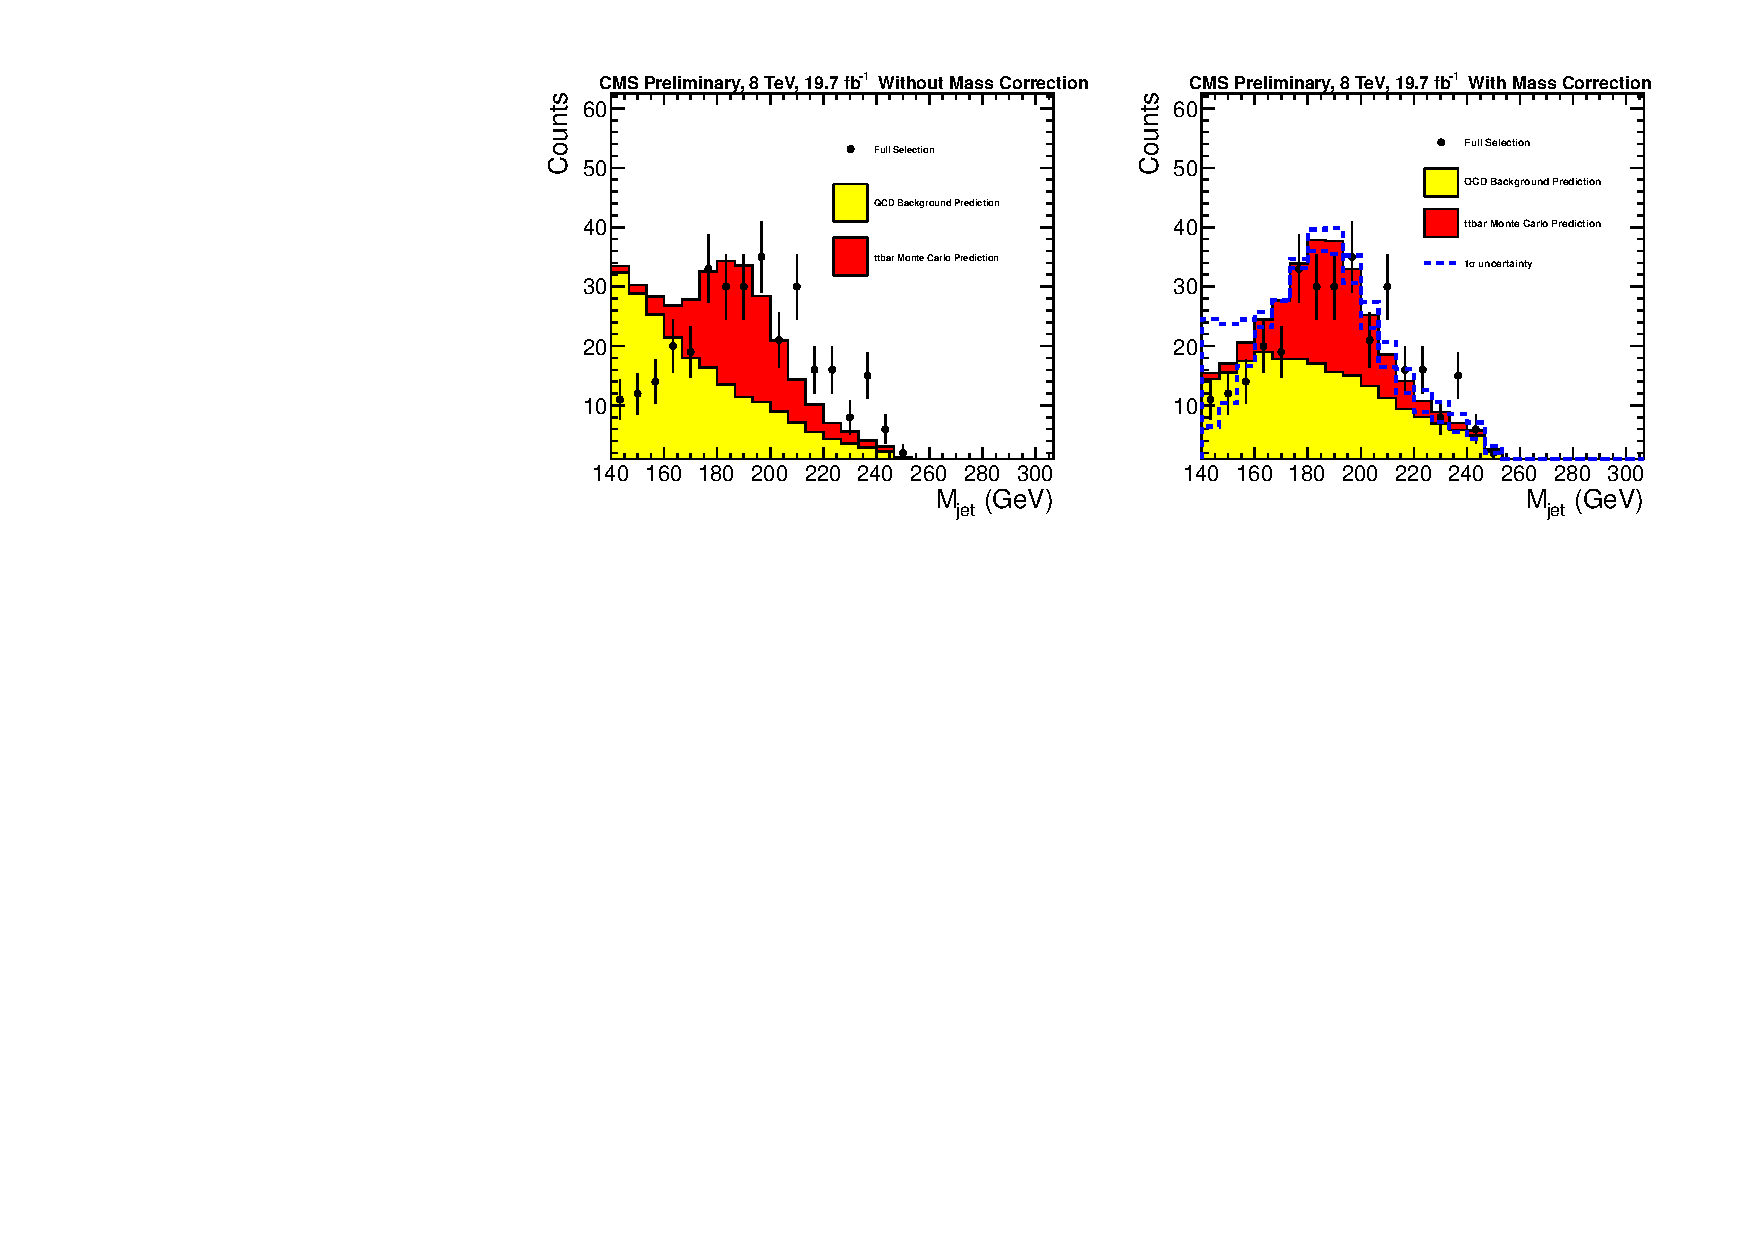
\includegraphics[width=1.0\textwidth]{AN-14-049/figs/tmasscomparison.pdf}}\\
\caption{Top candidate mass before (left) and after (right) the top candidate mass correction.  The selection for this plot is the full selection in the signal region.}
\label{figs:bsdatatmass}
\end{figure}

\begin{figure}[Htcb]
\centering
\subfigure{\label{figs:bsqcdtmass}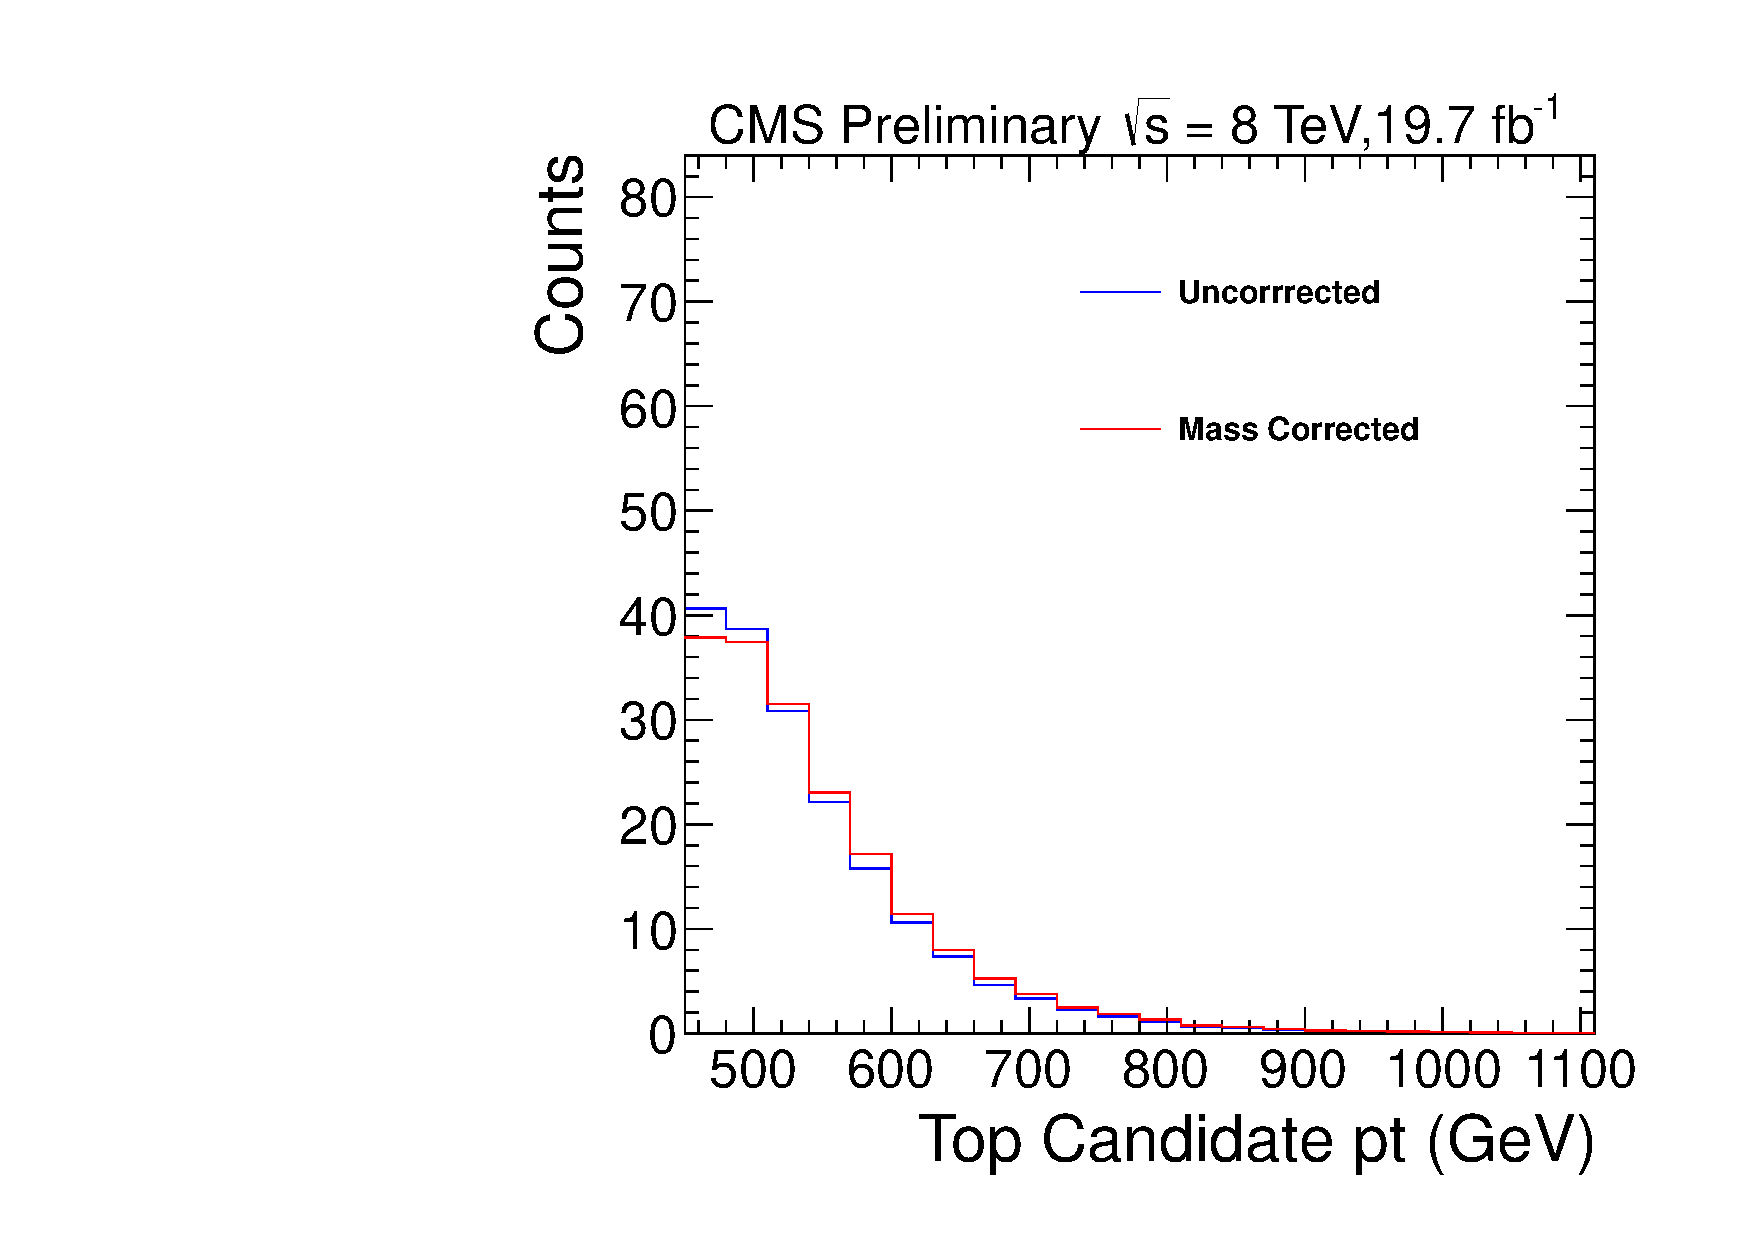
\includegraphics[width=.6\textwidth]{AN-14-049/figs/Mmeffecttpt.pdf}}\\
\subfigure{\label{figs:bsmodmassplot}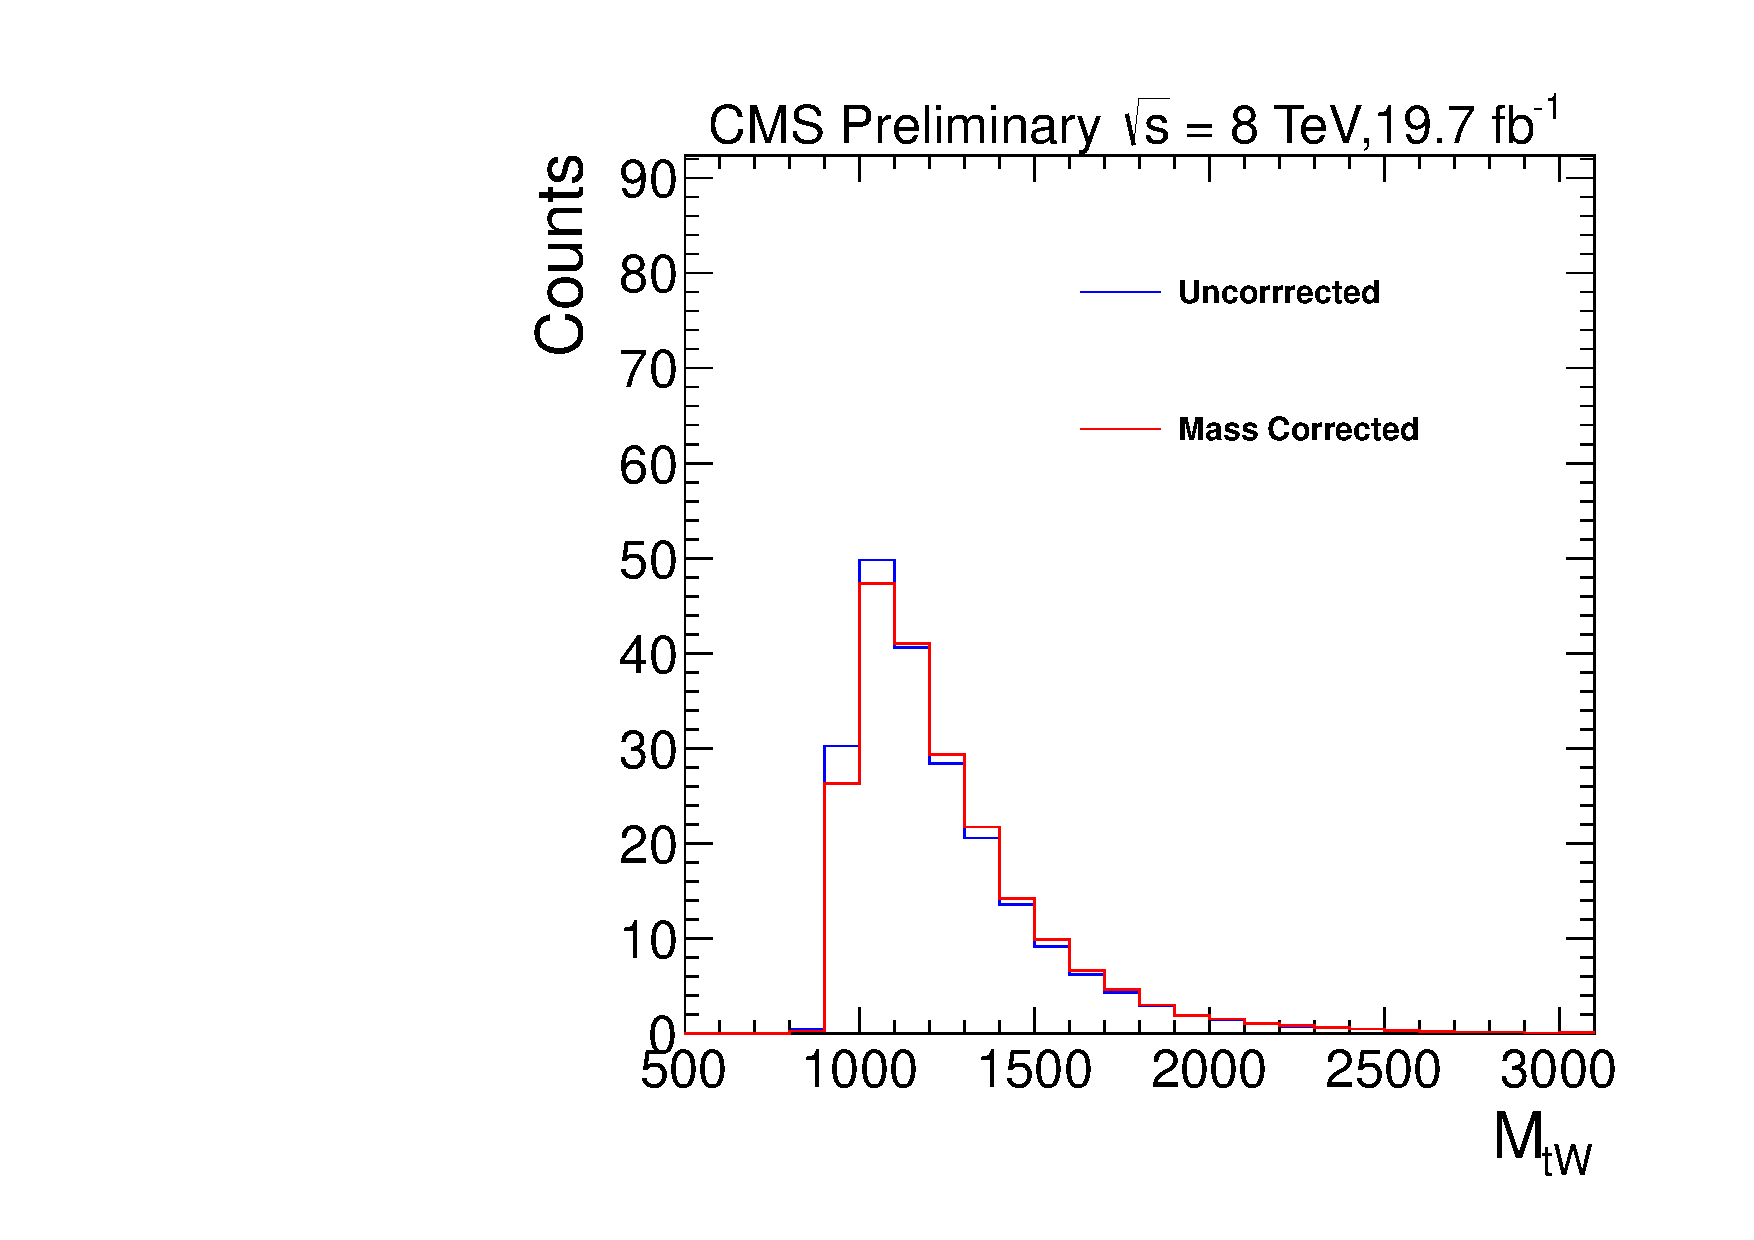
\includegraphics[width=.6\textwidth]{AN-14-049/figs/MmeffectMtw.pdf}}
\caption{A plot of the QCD background estimate before and after the top mass correction.  the top plots show the effect on top $\pt$, and the bottom plot shows the effect on $M_{tW}$.}
\label{figs:bsmodmasseffect}
\end{figure}





\section{Sideband Closure}
\label{sec:bssecondsideband}
In order to investigate the applicability and versatility of the QCD background estimation in data, we apply the top-mistagging rate to a control region of our 
W-tagging selection.  We define the following W-tagging sideband:

\begin{itemize}
\item {\bf Jet Mass}  $\mathrm{\boldmath 30~\GeV < m_{\text{jet}} < 70~\GeV~or~100~\GeV < m_{\text{jet}} < 130~\GeV }$ 
\item {\bf N-subjettiness} $\mathrm{\boldmath \tau_2/\tau_1 \geq 0.5}$ 
\end{itemize}
This sideband does not overlap with the control region used to extract the top-mistagging rate due to the inverted N-subjettiness window.
The selection has a lower yield of $\ttbar$ than the full selection, making it ideal for investigating the QCD background contribution.  
The closure test can be seen in Figure \ref{figs:bsNewMtbSB2}.  The termination of the W candidate mass requirement at 130 $\GeV$ is due to the fact that
above this region there is an increased yield of fully merged tops that pass the W-tagging sideband selection, which makes this region important for pinning 
down the $\ttbar$ normalization.

\begin{figure}[Htcb]
\centering
\subfigure{\label{figs:bsNewMtbSB21}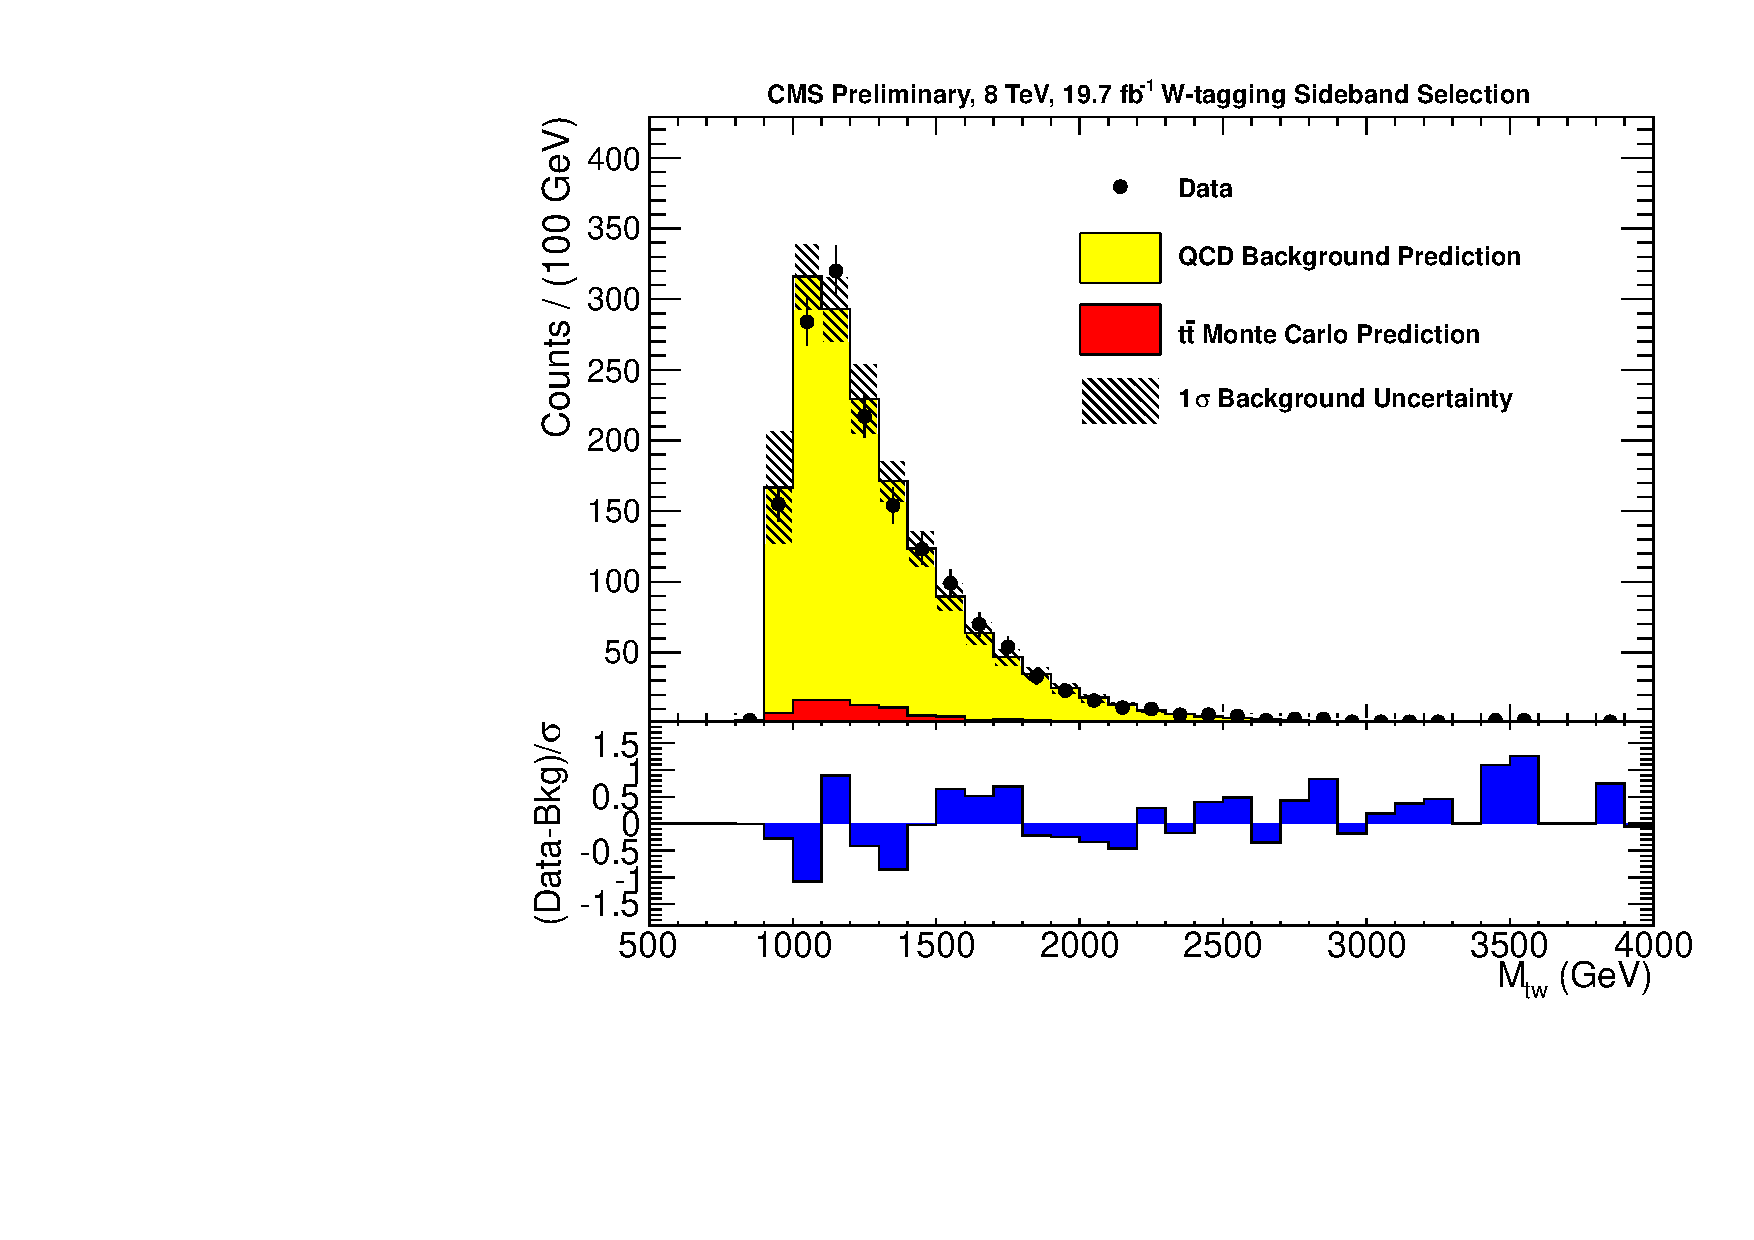
\includegraphics[width=0.7\textwidth]{AN-14-049/figs/MtwvsBkgwsbBifPoly_fit.pdf}}\\
\subfigure{\label{figs:bsNewMtbSB22}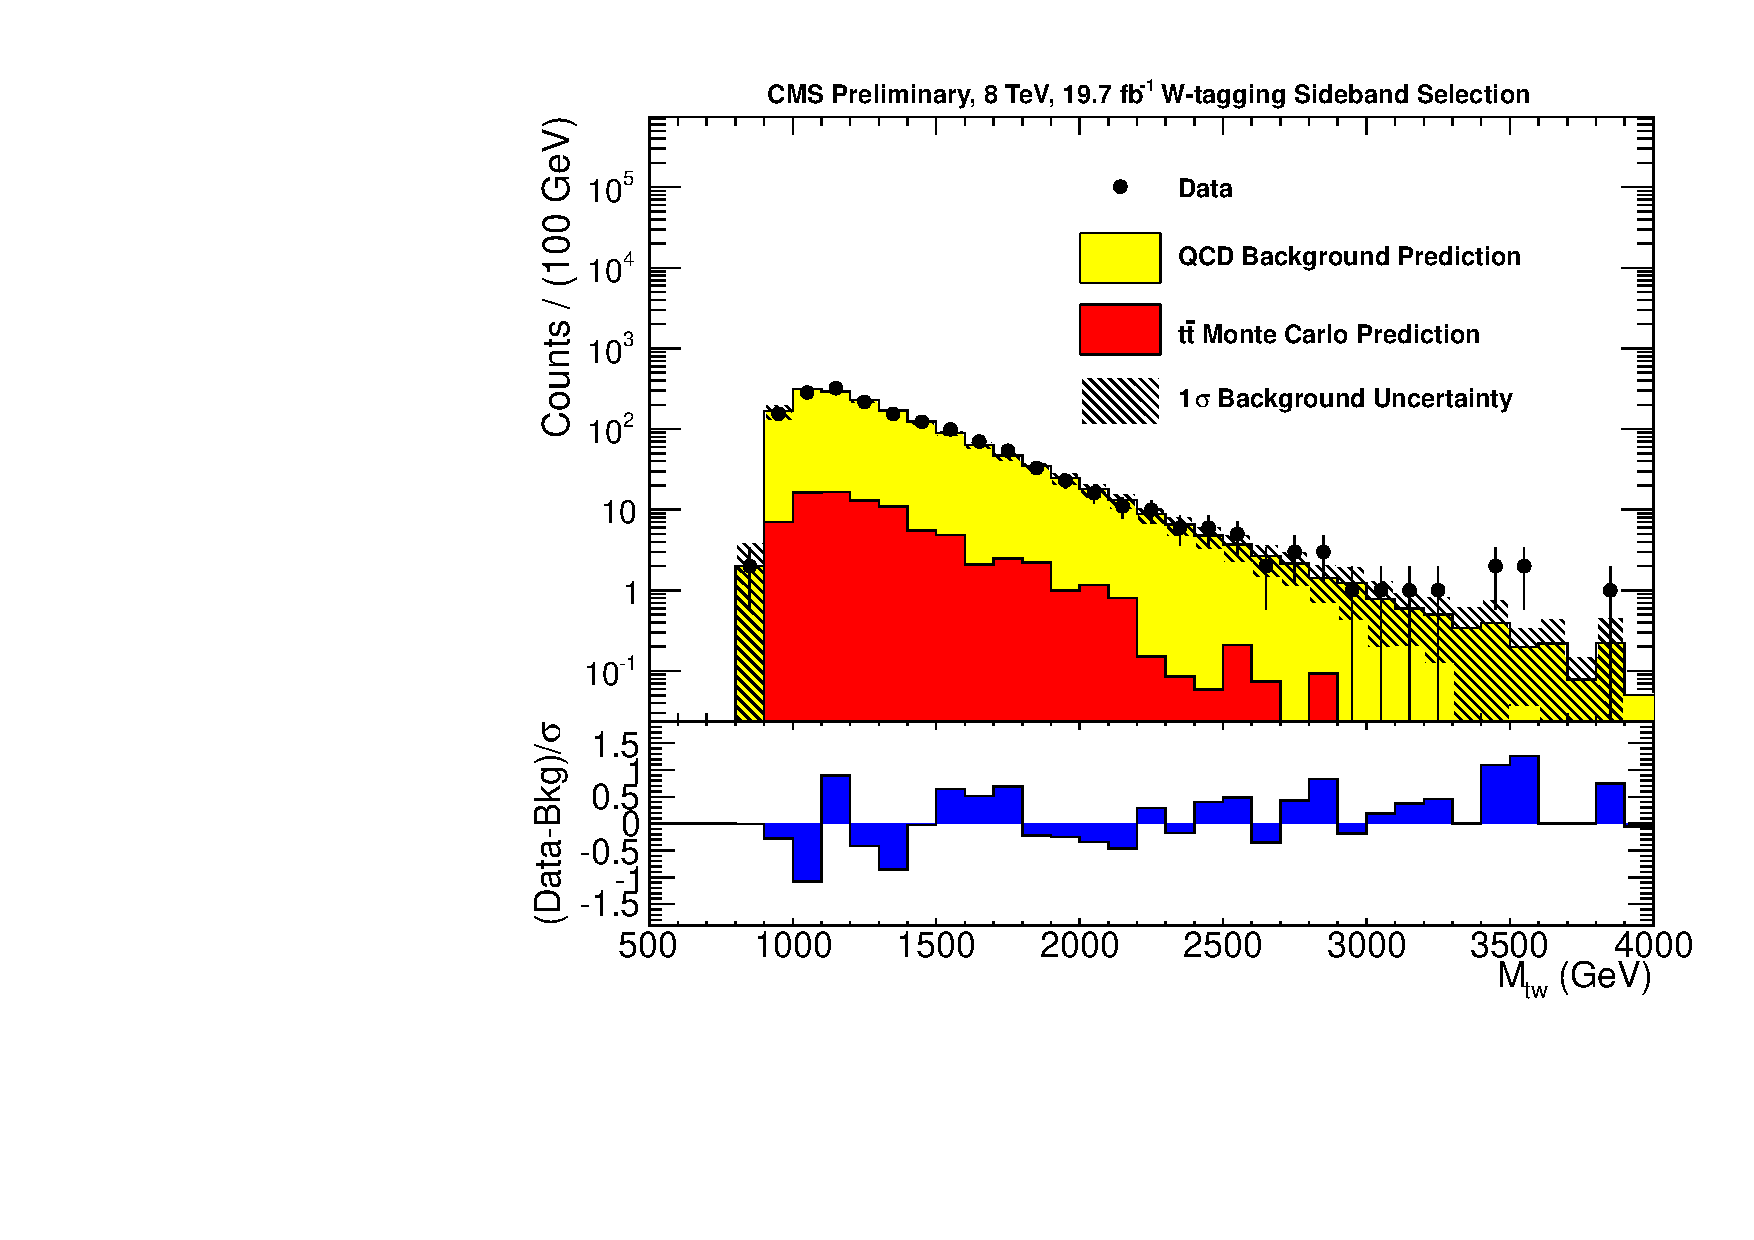
\includegraphics[width=0.7\textwidth]{AN-14-049/figs/MtwvsBkgwsbsemilogBifPoly_fit.pdf}}
\caption{A plot of $M_{tW}$ in the W-tagging sideband selection.  The top and bottom plots are the same but with linear and log y-axis scale.}
\label{figs:bsNewMtbSB2}
\end{figure}

\section{Deriving the Normalization of the SM $\ttbar$ Production}
\label{sec:bsttbarsideband}
In order to study the contribution from $\ttbar$ to the full background estimate, 
we investigate the following control region:
\begin{itemize}
\item {\bf Jet Mass}   $\mathrm{m_{\text{jet}} > 130~\GeV}$ 
\item {\bf N-subjettiness} $\mathrm{\boldmath \tau_2/\tau_1 \geq 0.5}$ 
\end{itemize}
This selection has an amplified $\ttbar$ fraction and is statistically independent from all other sidebands in the analysis.    
We extract the $\ttbar$ normalization by comparing the QCD background (extracted using the same top-mistagging rate as the signal region) and $\ttbar$ Monte Carlo to the selection in data.
%Here, the $\ttbar$ template is scaled to theory cross section using Monte Carlo to data scale factors used in the signal region except the W-tagging scale factor which is replaced by the W-mistagging scale factor described in section \ref{sec:bsCRSF}.  
The fit allows the QCD background template to move only within its errors, whereas the normalization on $\ttbar$ is unconstrained. 
We use the top candidate mass spectrum for fitting, which minimizes the correlation between the 
QCD and $\ttbar$ templates within the fit due to the top mass peak. This fit can be seen in Figure \ref{figs:bsttbarfit}.  For this maximum likelihood fit we use the Theta package.

$\ttbar$ is subtracted from the numerator and denominator of the top-mistagging rate when extracting the QCD background estimate in the signal region.  
Additionally, $\ttbar$ contamination (se section \ref{sec:bsttSubtraction}) is subtracted from the QCD background estimate after the application of the top-mistagging rate.  
This $\ttbar$ contamination is estimated by weighting the pre top-tagged $\ttbar$ selection by the top-mistagging rate.  The fitting procedure needs to implement both of these subtractions 
in order to isolate the $\ttbar$ normalization constant, because through these mechanisms the QCD shape is dependent on the $\ttbar$ normalization.

The fit implements the $\ttbar$ subtraction in the QCD estimate by fitting un-subtracted QCD to the $\ttbar$ full selection.  
The output of the fitter is then corrected by  
(1+S/F), where S/F is the ratio of the number of events in $\ttbar$ subtraction to the $\ttbar$ full selection. 

The fit additionally implements $\ttbar$ subtraction in creation of the top-mistagging rate by creating two QCD components.  One component is anticorrelated 
with the $\ttbar$ normalization factor, and the other is independent of this normalization factor.  The anticorrelated QCD component fraction of the QCD estimate 
is taken as the difference of the QCD estimate with and without $\ttbar$ subtraction.  The independent QCD component fraction of the QCD estimate is taken as the 
difference of the QCD estimate and the anticorrelated component.  

This study suggests after all scale factors applied in the analysis, the $\ttbar$ contribution needs to be scaled by $0.79 \pm 0.17$.  
This normalization is used for all $\ttbar$ distributions in the analysis, and the uncertainty is then the full normalization uncertainty for $\ttbar$.

\begin{figure}[htcb]
\centering
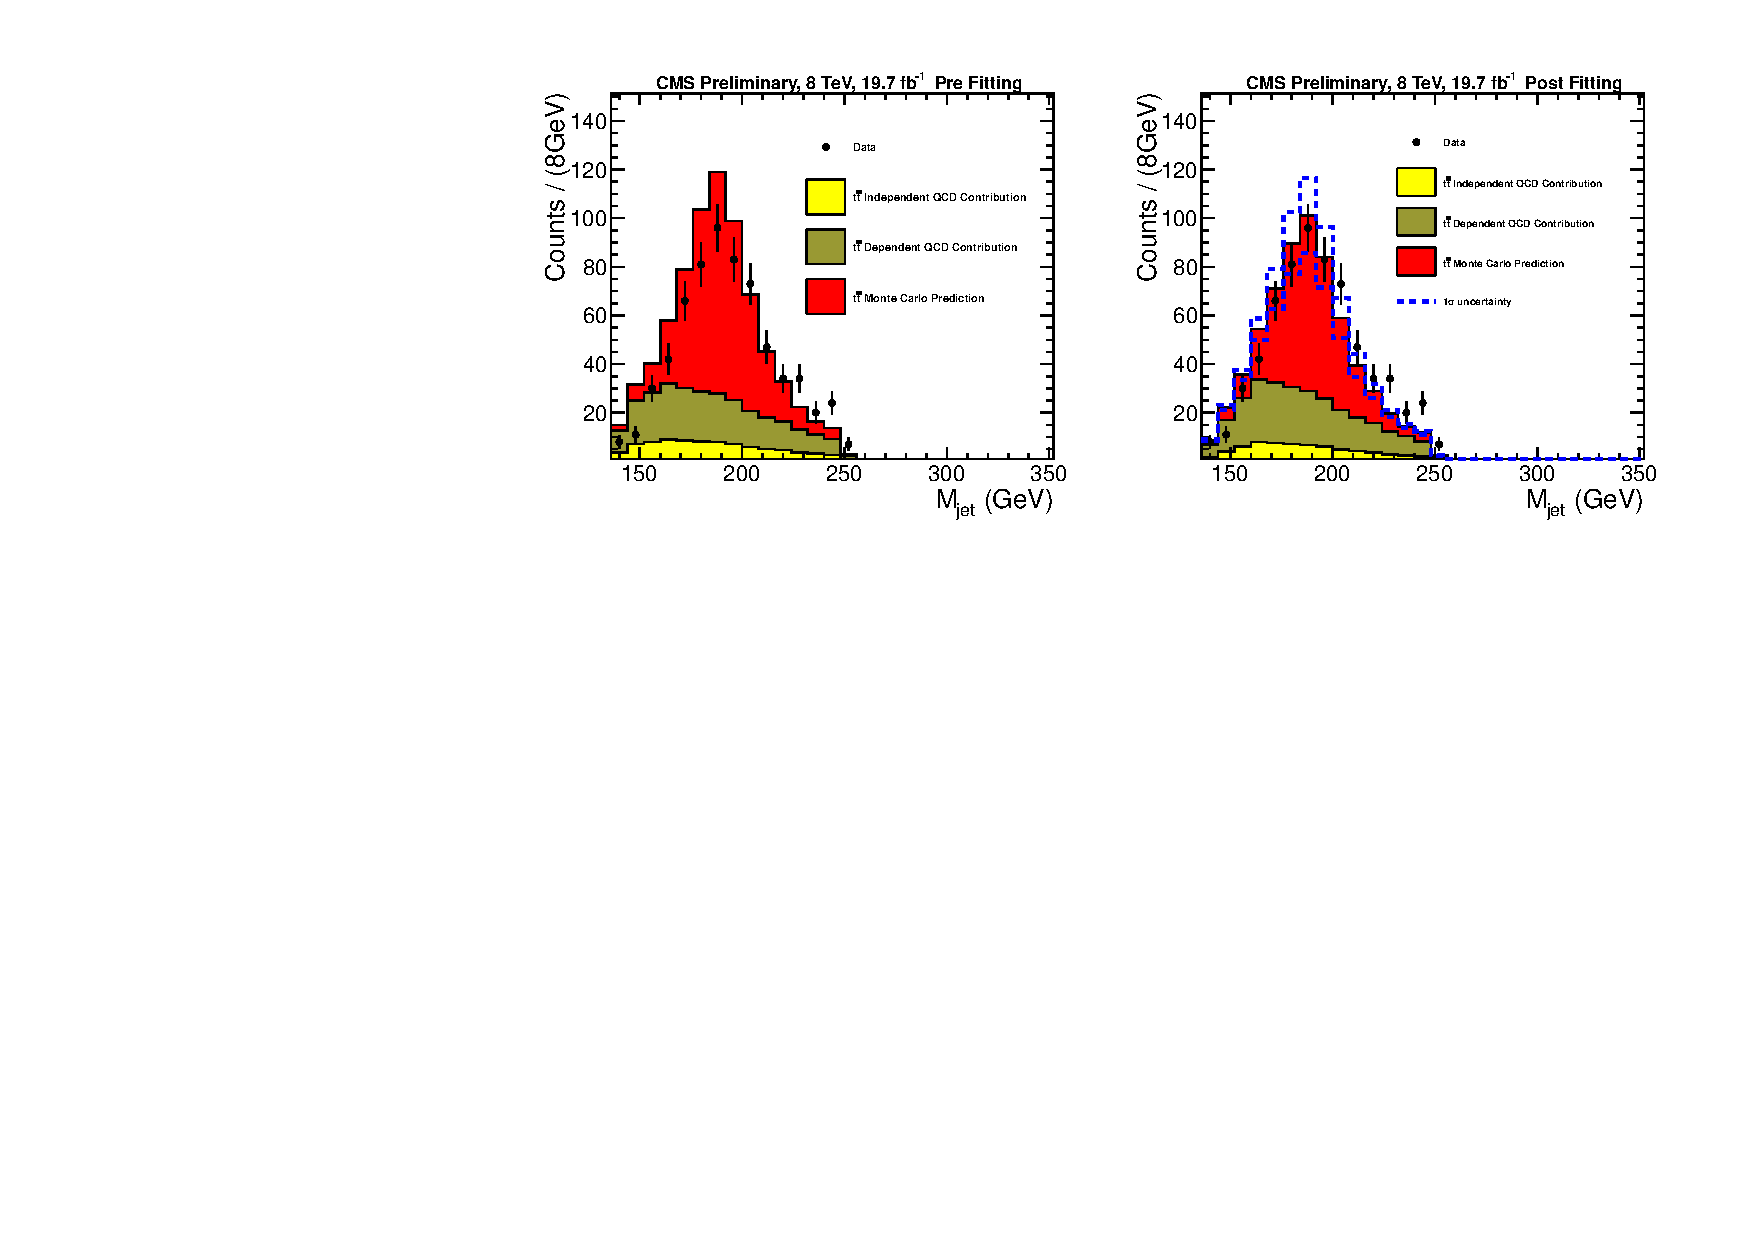
\includegraphics[width=1.0\textwidth]{AN-14-049/figs/ttbarfittingfromtheta.pdf}
\caption{top candidate jet mass as extracted from the high mass W-tagging sideband.  Pre fraction fit (left) and post fraction fit (right).  The two QCD components use identical template shapes,
but the normalization is such that one component can be considered independent from $\ttbar$, and the other will be anticorrelated $\ttbar$ normalization constant. }
\label{figs:bsttbarfit}
\end{figure}

\section{Control Region Scale Factors}
\label{sec:bsCRSF}
The W-tagging control regions mentioned in sections \ref{sec:bsttbarsideband} and \ref{sec:bssideband} are used for measurements that impact the background estimate in the signal region.  
These  inverted selections do not have known scale factors, so we derive them using the semileptonic sample mentioned in section \ref{sec:bssubjetSF}.  The scale factor for the control region mentioned in 
section \ref{sec:bssideband} is determined to be $0.97 \pm 0.06$, and the scale factor for the control region mentioned in section \ref{sec:bsttbarsideband} is $1.12 \pm 0.09$.  

The scale factors are a product of the W candidate mass window scale factor and the $\tau_2/\tau_1$ window scale factor.  The W candidate mass used for this measurement can be seen in figure \ref{figs:bsmassCRSF}.
Given the mass window, we then investigate $\tau_2/\tau_1$ for the jet.  This can be seen in figure \ref{figs:bsNsubCRSF1} for the scale factor of the control region mentioned in section \ref{sec:bssideband} and 
figure \ref{figs:bsNsubCRSF1}  for the scale factor of the control region mentioned in section \ref{sec:bsttbarsideband}.

\begin{figure}[htcb]
\centering
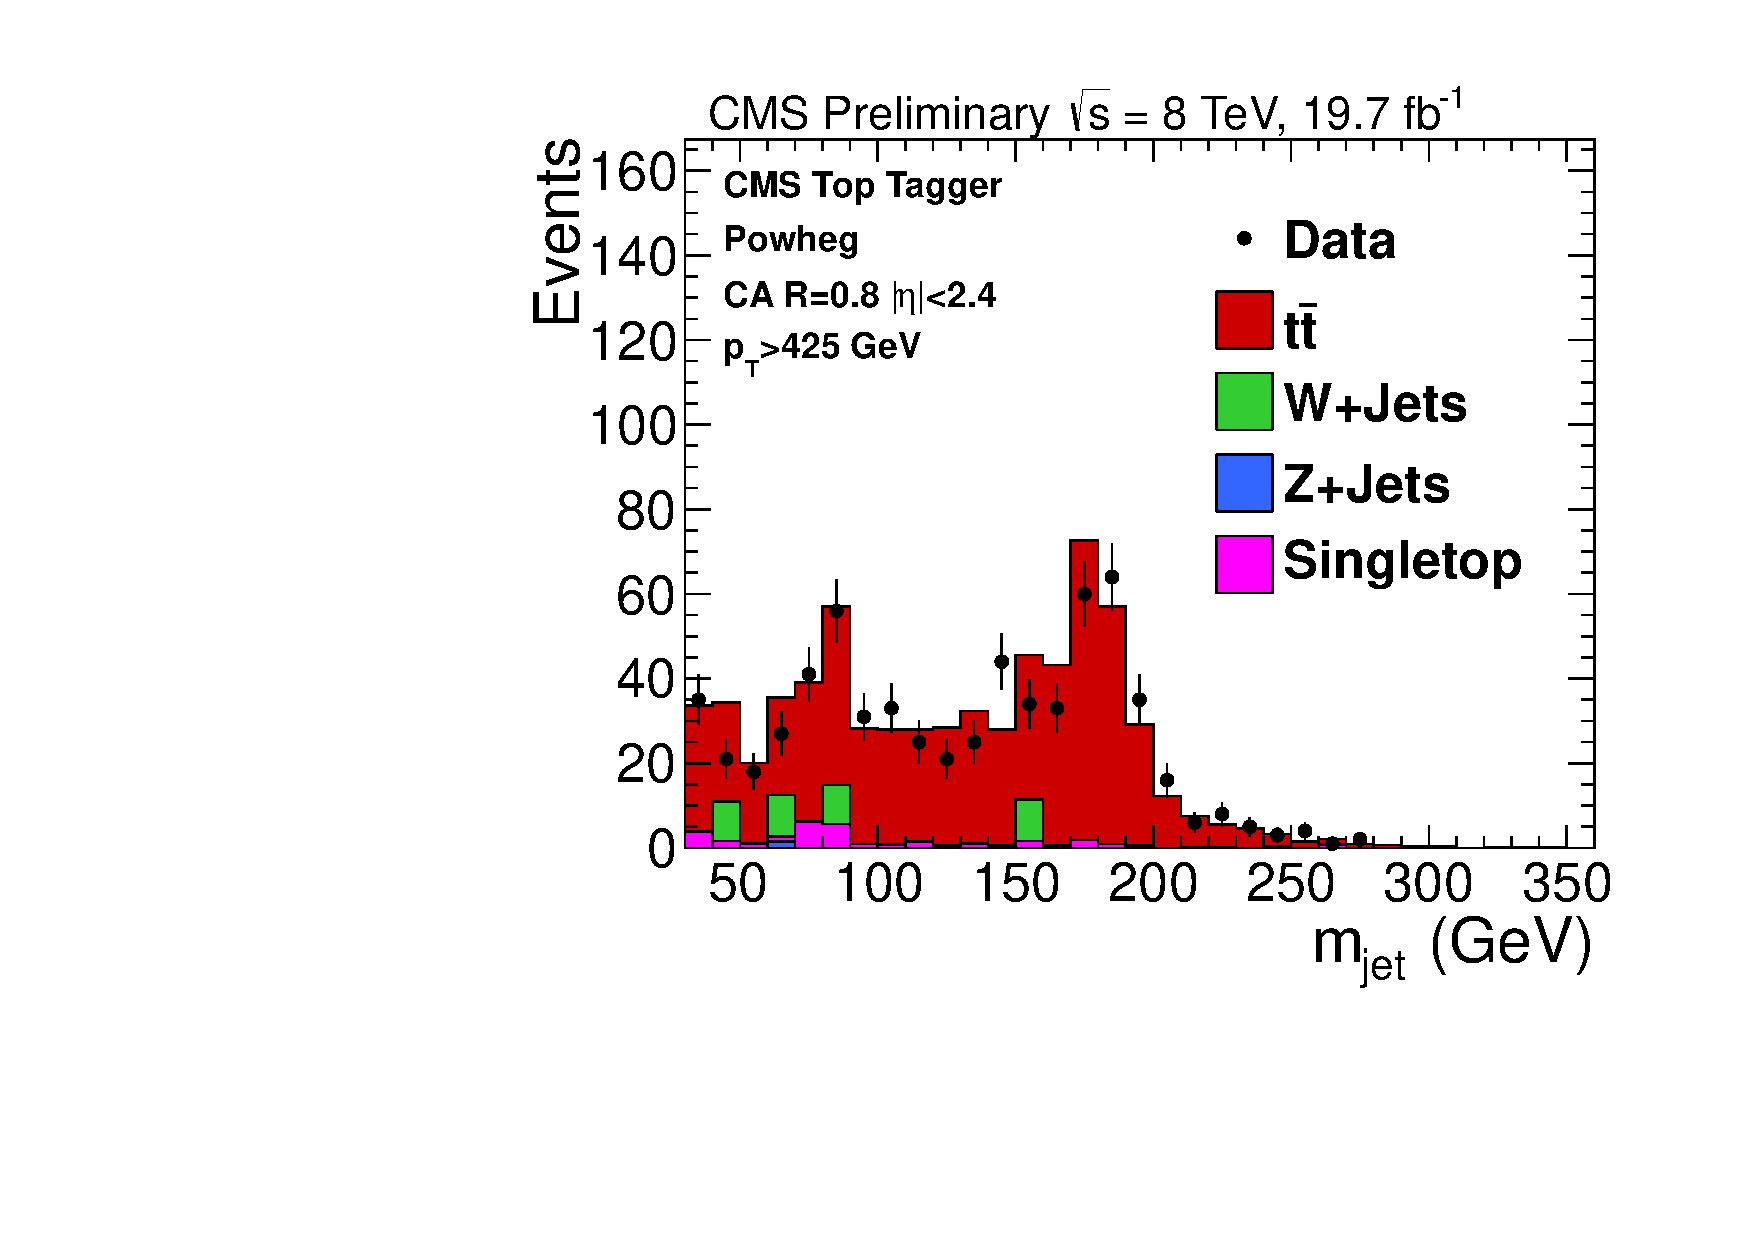
\includegraphics[width=1.0\textwidth]{AN-14-049/figs/semiLepMassbstar_t1TopMass_POWHEG_TTWeight.pdf}
\caption{A plot of W candidate jet mass used for determination of the control region scale factors. }
\label{figs:bsmassCRSF}
\end{figure}

\begin{figure}[htcb]
\centering
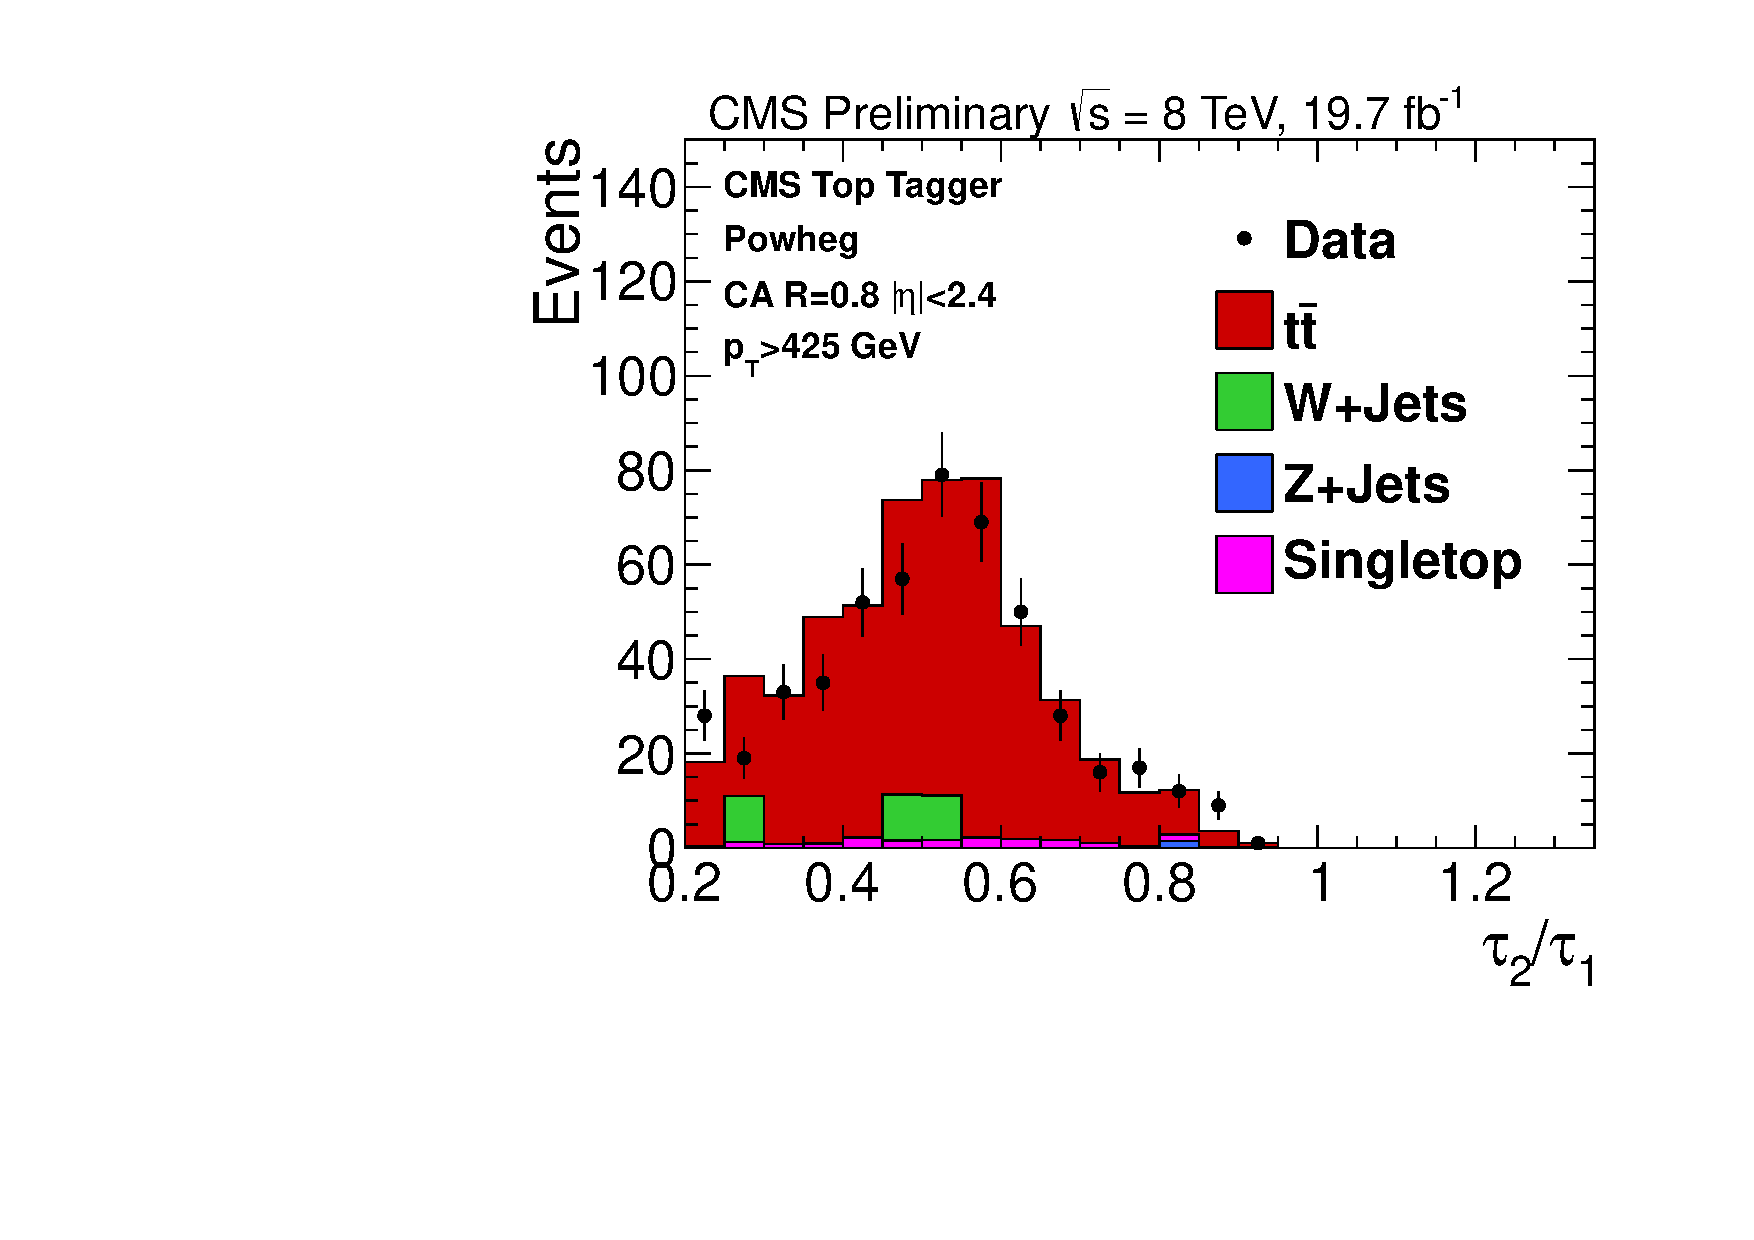
\includegraphics[width=1.0\textwidth]{AN-14-049/figs/semiLepMassbstar1_t1Tau21_POWHEG_TTWeight.pdf}
\caption{A plot of $\tau_2/\tau_1$ used for determination of the scale factor for the control region used for extracting the top-mistagging rate. }
\label{figs:bsNsubCRSF1}
\end{figure}

\begin{figure}[htcb]
\centering
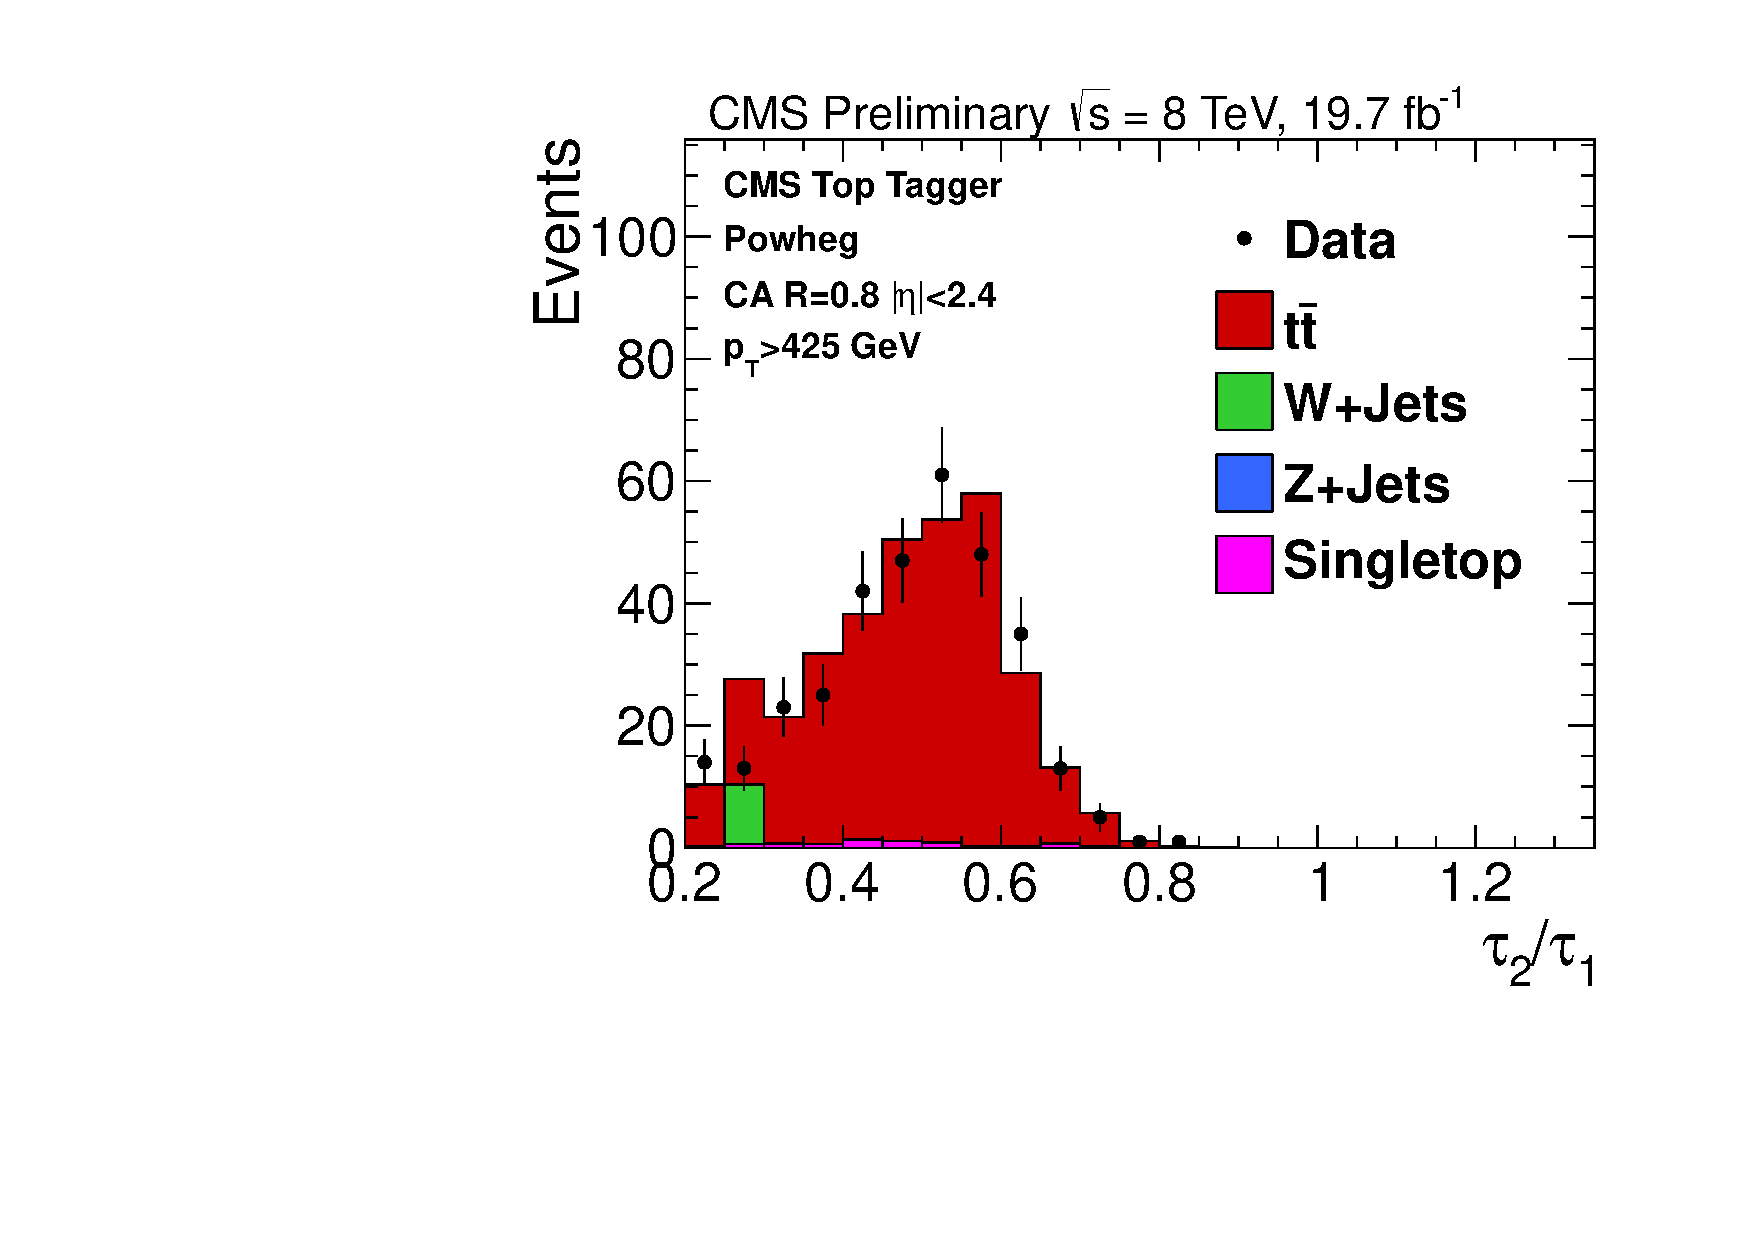
\includegraphics[width=1.0\textwidth]{AN-14-049/figs/semiLepMassbstar_t1Tau21_POWHEG_TTWeight.pdf}
\caption{A plot of $\tau_2/\tau_1$ used for determination of the scale factor for the control region used for extracting the $\ttbar$ normalization. }
\label{figs:bsNsubCRSF}
\end{figure}



